\chapter{Graphs and networks} % (fold)
\label{cha:graphs_and_networks}



The networks studied in this document can be represented by a single graph.
In general, the term \textit{graph} is used for the mathematical object defined below and the term \textit{network} for some model that relies on one (or more) graphs.

We begin by defining some terminology and proceed to described models of random graphs.

\section{Terminology and essential results} % (fold)
\label{sec:definitions_and_essential_results}

\begin{definition}A graph $G$ is a tuple
\begin{equation}
G = (V,E),
\end{equation}
\noindent where $V$ is the set of vertices (or nodes), and $E$ is the set of edges (or links).
Each edge connects exactly one pair of vertices, and a vertex-pair can be connected by maximally one edge, i.e., multi-connections are not allowed.
Let furthermore $n$ denote the number of vertices $n = |V|$ and $L$ the number of edges $L = |E|$.
\end{definition}


In this thesis, the set $V$ will correspond to the set of obligors in a portfolio, and $E$ to the interdependencies between the obligors.
In the case of a social network, for example, $V$ would be the set of persons and $E$ could mean that two persons (nodes) are acquainted (connected) with each other.

\begin{definition}A weighted graph $G$ is a graph where a number $x \in \R$ can be assigned to an element of $E$.\end{definition}

\begin{definition}An unweighted graph $G$ is a graph where no number is assigned to an element of $E$.\end{definition}


\begin{definition}The adjacency matrix $A$ of a graph $G = (V,E)$ is a matrix of size $n\times n$, such that each element $a_{ij}$ of the matrix is given by
\begin{equation}
	a_{ij} = \begin{cases}
	1 & \text{if there is an edge between $i$ and $j$, i.e. } } \{i,j\} \in E\\
	0 & \text{otherwise}
	         \end{cases}
\end{equation}
If $G$ is a weighted graph, then the 
\begin{equation}
	a_{ij} = \begin{cases}
	w_{ij} & \text{if there is an edge between $i$ and $j$ with weight $w_{ij}$ } }\\
	0 & \text{otherwise}
	         \end{cases}
\end{equation}
\end{definition}

\begin{remark}Throughout this document we will be concerned with graphs without self-edges, so that $\forall i, \, a_{ii} = 0$.\end{remark}

\begin{definition}An undirected graph $G$ is a graph where its adjacency matrix $A$ is symmetric, i.e. $\forall i,j, \, a_{ij} = a_{ji}$.\end{definition}

\begin{definition}A connected component (or just component) of an undirected graph $G = (V,E)$ is a subgraph $G' = (V', E')$ where:
\begin{enumerate}[(i)]
	\item $V'$ and $E'$ are subsets of $V$, $E$ respectively
	\item any two vertices $a,b in V'$ are connected to each other by a sequence of edges $[ e_1,\ldots, e_k]$ such that $e_1, \ldots, e_k \in E'$
	\item given a vertex $a \in V'$, for all vertices $b$ such that ${a,b} \in V'$, $b \in E'$.
\end{enumerate}\end{definition}

\begin{definition}The degree $k_i$ of a node $i$ in an undirected graph $G$ is the sum of the  elements of the $i^{th}$ row (column) of its adjacency matrix $A$, i.e. $k_i = \sum_{j=1}^{j=n} a_{ij}$ .\end{definition}
\begin{remark}In case $G$ is unweighted, then the degree of node $i$ is equal to the number of edges that connect to that node. In case $G$ is weighted, then it corresponds to the sum of the weights of the edges that connect to that node.\end{remark}


\begin{definition}The degree matrix $D$ is a graph $G$ is an $n\times n $ matrix where its diagonal contains the degree of the corresponding vertices, i.e. where $$d_{ij} = \begin{cases}
    k_i & \text{if } i = j \\
	0 & \text{ otherwise.} 
\end{cases}$$
\end{definition}

\begin{definition}The Laplacian~\footnote{Please note that there may be similar alternative definitions of the Laplacian matrix of a graph, but its properties equivalent w.r.t. the requirements for this thesis.}  matrix $L$ of a graph $G$ is given by $L = D - A$, where $D$ is the degree matrix and $A$ the adjacency matrix, as defined above.
\end{definition}

\begin{remark}The graph Laplacian turns up in a large variety of places in network modelling, including diffusion processes, random walks, graph partitioning and, the most important for the purpose of this thesis, network connectivity.\end{remark}

There is, in fact, a connection between the eigenvectors of the Laplacian matrix of a graph and its connected components, which will allow us to easily compute the component structure of particular instances of graphs.
In fact, a graph $G$ with multiple connected components $C_k$ will have a Laplacian matrix $L$ that is a block diagonal matrix.
After reordering of the vertices, each block in this matrix will be the corresponding Laplacian matrix for each component $C_k$.
\begin{theorem}
Consider a graph $G$, with a Laplacian matrix $L$. Then,
\begin{enumerate}[(i)]
	\item all eigenvalues of $L$ ${\displaystyle \lambda _{0}\leq \lambda _{1}\leq \cdots \leq \lambda _{n-1}} \lambda_0 \le \lambda_1 \le \cdots \le \lambda_{n-1}$ are $\ge 0$
	\item $\lambda_j = 0 \iff $ the corresponding eigenvector defines a connected component.
\end{enumerate}
\end{theorem}
\begin{proof}The proof is left here undone, as it can be found in most books on networks, e.g.~\cite{newman2010networks}.\end{proof}
\begin{remark}

In order to find the connected components of a graph, one can compute the null-eigenvalues and eigenvectors of its Laplacian matrix.

\end{remark}
\begin{example}{\noindent Example: }We consider the following example of a graph
\end{example}
\begin{figure}[hb]
	\centering
	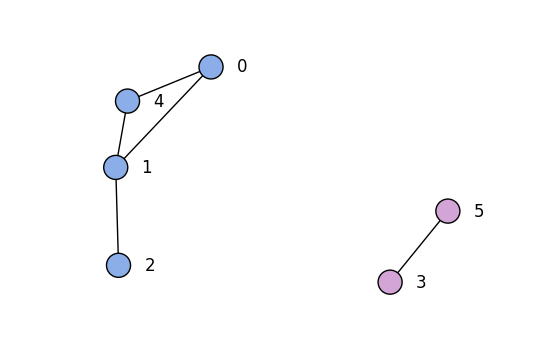
\includegraphics[scale=0.8]{figures/2_example_graph.png}
	\caption{Example graph with 2 components and 6 nodes.}
	\label{fig:example_graph}
\end{figure}
which has following (rows and columns 4,5 permutated) adjacency matrix
$$
A = \begin{bmatrix}
  0 & 1 & 0 & 1 & 0 & 0\\
  1 & 0 & 1 & 1 & 0 & 0\\
  0 & 1 & 0 & 0 & 0 & 0\\
  1 & 1 & 0 & 0 & 0 & 0\\
  0 & 0 & 0 & 0 & 0 & 1\\
  0 & 0 & 0 & 0 & 1 & 0\\
\end{bmatrix}
$$
\noindent and Laplacian matrix
% $${\begin{pmatrix}0&1&0&0&1&0\\1&0&1&0&1&0\\0&1&0&1&0&0\\0&0&1&0&1&1\\1&1&0&1&0&0\\0&0&0&1&0&0\\\end{pmatrix}}$$
$$
L = \begin{bmatrix}
  2 & -1 & 0 & -1 & 0 & 0\\
  -1 & 3 & -1 & -1 & 0 & 0\\
  0 & -1 & 1 & 0 & 0 & 0\\
  -1 & -1 & 0 & 2 & 0 & 0\\
  0 & 0 & 0 & 0 & 1 & -1\\
  0 & 0 & 0 & 0 & -1 & 1\\
\end{bmatrix}
$$
The block- structure of the Laplacian matrix is well visible and easy to correspond to the community structure in the plotted graph.

% section definitions_and_essential_results (end)


\section{Random graphs} % (fold)
\label{sec:random_graph_model}

A random graph is a graph that is generated by randomly sampling from a collection of graphs, i.e. a random variable defined in a probability space with a probability distribution.
\begin{definition}
The Erd\"os-R\'enyi random graph $G_{n, p}$ is the random graph containing $n$ nodes obtained by connecting pairs of vertices with an edge with probability $p$. Each edge exists independently with the same probability.
\end{definition}
Under this model, the probability of any simple graph $G$, i.e. without multiple edges or self-loops, with $n$ nodes and $m$ edges is given by
$$P(G) = p^m (1-p)^{\binom{n}{2} - m}$$


This model was studied by the Hungarian mathematicians Paul Erd\"os (1913-1996) and Alfr\'ed R\'enyi (1921-1970), and has lead to a large corpus of research on random graphs.
As with other models studied in this thesis, statements made about the model are statements made about the collection of graphs, rather than any specific instance of a graph.

\begin{figure}[tb]
	\centering
	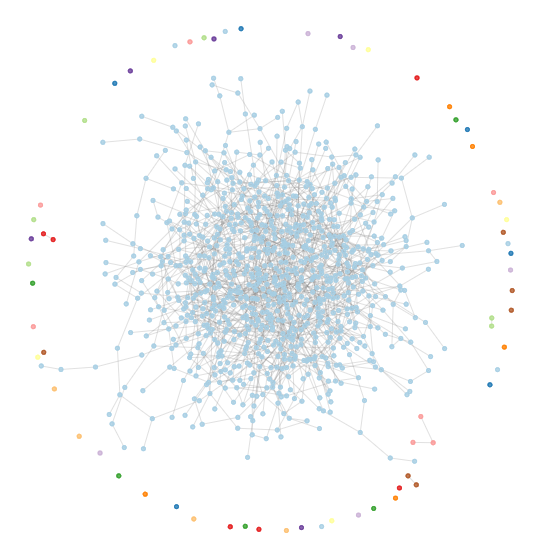
\includegraphics[width=10cm]{figures/gnp_hairball.png}
	\caption{Plot of a random graph with $n = 1000$ nodes, edge probability $p = 0.003$ and $c=3$. 
	Nodes belonging to the same connected component are coloured identically.
	We can see a dominating large component in the graph through the light blue nodes in the centre.
	The existence of this dominating component is described in section~\ref{sub:giant_component}.}
	\label{fig:hairball}
\end{figure}

The random graph model is especially interesting because several of its statistical properties can be derived analytically.
The properties of the networks it generates, however, differ substantially from those observed in real world networks~\cite{Albert:2002p4071}.

\subsection{Mean degree and degree distribution} % (fold)
\label{ssub:mean_degree_and_degree_distribution}

In the random graph model, the existence of any edge is independent from each other and solely determined by the same probability value $p$.
As such, the probability of a graph with $m$ edges drawn from the $G(n,p)$ model is given by a binomial distribution choosing $m$ edges out of a universe of $\binom{n}{2}$ edges
\begin{equation}
	P(m) = \binom{\binom{n}{2}}{m} p^m (1-p)^{\binom{n}{2}-m}
\end{equation}
Therefore, the expected number of edges is given by
\begin{equation}
	\mean{m} = \sum^{\binom{n}{2}}_{m=0} m P(m) = \binom{n}{2} p
\end{equation}
% In the course of this document, we will be not only interested on the properties of the graph itself, but also on how they build from the individual properties of the edges and nodes.
Using this result, we can derive the expected mean node degree $c$ in a graph
\begin{equation}
	c = \sum^{\binom{n}{2}}_{m=0} \frac{2m}{n} P(m) = \frac{2}{n} \binom{n}{2} p = (n-1) p,
\end{equation}

More generally, we can not only derive the mean, but also the entire distribution of the node degree.
In fact, any node in the graph is connected with independent probability $p$ to any of the remaining $n-1$ nodes in the graph.
Hence, the probability of having a particular degree $k$, i.e. being connected to exactly $k$ other nodes, is $p^k (1-p)^{n-1-k}$.
Given that there are $\binom{n-1}{k}$ possible sets of $k$ vertices, the probability distribution of the node degree is given by
\begin{equation}
    \label{eq:degree_dist_naive}
	p_k = \binom{n-1}{k} p^k (1-p)^{n-1-k}
\end{equation}


We sometimes wish to consider not only small but also large networks.
When $n$ is assumed to be large, some useful approximations can be made, which render the model more analytically tractable.

When $n\rightarrow \infty$, we can rewrite
\begin{align}
	ln[(1-p)^{n-1-k}] &= (n-1-k) \ln\left( 1-\frac{c}{n-1} \right)\\
                      &\simeq (n-1-k) \frac{c}{n-1}\\
                      &\simeq -c,\\
\intertext{\noindent and therefore }
    (1-p) ^{n-1-k} & \simeq e^{-c}
\end{align}
\noindent by using the Taylor expansion of $\ln\left(1-\frac{c}{n-1}\right)$ and approximating to the first term.
These approximations hold exactly when $n\rightarrow \infty$, as does the following approximation when
\begin{align}
    \binom{n-1}{k} = \frac{(n-1)!}{(n-1-k)! k!} \simeq \frac{(n-1)^k}{k!}
\end{align}
By applying both approximations under the assumption that $n \rightarrow \infty$, we can rewrite equation~\vref{eq:degree_dist_naive} as follows
\begin{equation}
	p_k = \frac{(n-1)^k}{k!} p^k e^{-c} = e^{-c} \frac{c^k}{k!}
\end{equation}
which is the familiar Poisson distribution.

% subsection mean_degree_and_degree_distribution (end)Mean degree and degree distribution


\subsection{Giant component} % (fold)
\label{sub:giant_component}

Although very simple, the random graph model possesses one very interesting property: the sudden appearance of the so-called giant component by varying the mean degree $c$.
A giant component is a component whose size is proportional to the size of the network $n$, and its sudden appearance is called a \textit{phase transition}.

Consider the random graph $G_{n, p}$ with two extreme parametrisations:
\begin{itemize}
	\item[] $p = 0$, there are no edges in the graph, and therefore the largest component is of size $1$,
	\item[] $p = 1$ every vertex is connected with every other vertex, and so the largest connected component has size $n$. 
\end{itemize}
Under $p=1$, the size of the largest component grows with the network.
This is called a giant component, and its size can be computed exactly in the limit of a large network size.

\begin{definition}
Let $u$ denote the average fraction of vertices not in the giant component. Let $S$ be the reciprocal of $u$, $S = 1 - u$, i.e. the average relative size of the giant component.
\end{definition}
\noindent By definition the giant component exists if and only if $u<1$. Suppose that, under the $G(n,p)$, vertex $i$ does not belong to the giant component.
Consider another vertex $j$.
Either
\begin{enumerate}[i)]
	\item $i$ and $j$ are not connected with probability $1-p$, or
	\item there is an edge between $i$ and $j$ and $j$ also does not belong to the giant component, which has a probability of $pu$.
\end{enumerate}
As such, the probability that there is an edge $(i,j)$ is $1-p + pu$.
If we now consider every node in the graph, then the probability that node $i$ is not in the giant component is $u$, and depends on it only being connected to nodes not being in the giant component.
Since every edge in the graph exists independently, then we have
\begin{equation}
	u = (1- p + pu)^{n-1} = \left[ 1 - \frac{c}{n-1} (1-u)\right]^{n-1}
\end{equation}
If we take the logarithm of both sides, 
\begin{equation}
	\ln u = \ln\left[ 1 - \frac{c}{n-1} (1-u)\right]^{n-1} = (n-1) \ln\left( 1-\frac{c}{n-1} (1-u)\right)
\end{equation}
When $n$ is large, $\frac{c}{n-1}$ is very small, so that we following approximation holds
\begin{equation}
	\ln\left( 1-\frac{c}{n-1} (1-u)\right) \approx - \frac{c}{n-1} (1-u)
\end{equation}
and therefore,
\begin{equation}
	\ln u \approx - c (1-u)
\end{equation}
By taking the exponential of both sides, we can write it as
\begin{equation}
	u \approx e^{-c(1-u)}
\end{equation}
Alternatively, one can consider the reciprocal of $u$, i.e. the fraction $S$ of nodes that do belong to the giant component.
\begin{equation}
    \label{eq:s_naive}
	S = 1 - e^{-cS}
\end{equation}
This equation has a trivial solution at $S = 0$, which is the only solution if $c \le 1$, i.e. there is no giant component if $c \le 1$.
For $c > 1$, there is not only the trivial solution but also another solution at $S > 0$.
\cite{newman2010networks} shows that the non-trivial solution best describes the giant component.

\noindent Although very simple, equation~\ref{eq:s_naive} has no closed-form solution.
It can be expressed through the \Lambert $W$-function~\footnote{The Lambert-W function is a set of functions representing the inverse relation of the function $f(z) = z e^{z}$ where $z$ is a complex number, i.e. {\displaystyle\, z=f^{-1}(ze^{z})=W(ze^{z})}}
\begin{equation}
S = 1 + \frac{W(-c e^{-c})}{c}
\label{eq:s_giant_component_lambert}
\end{equation}
\noindent, for which there are standardized numerical software module, e.g.~\cite{sympy}.

\begin{figure}[tb]
	\centering
	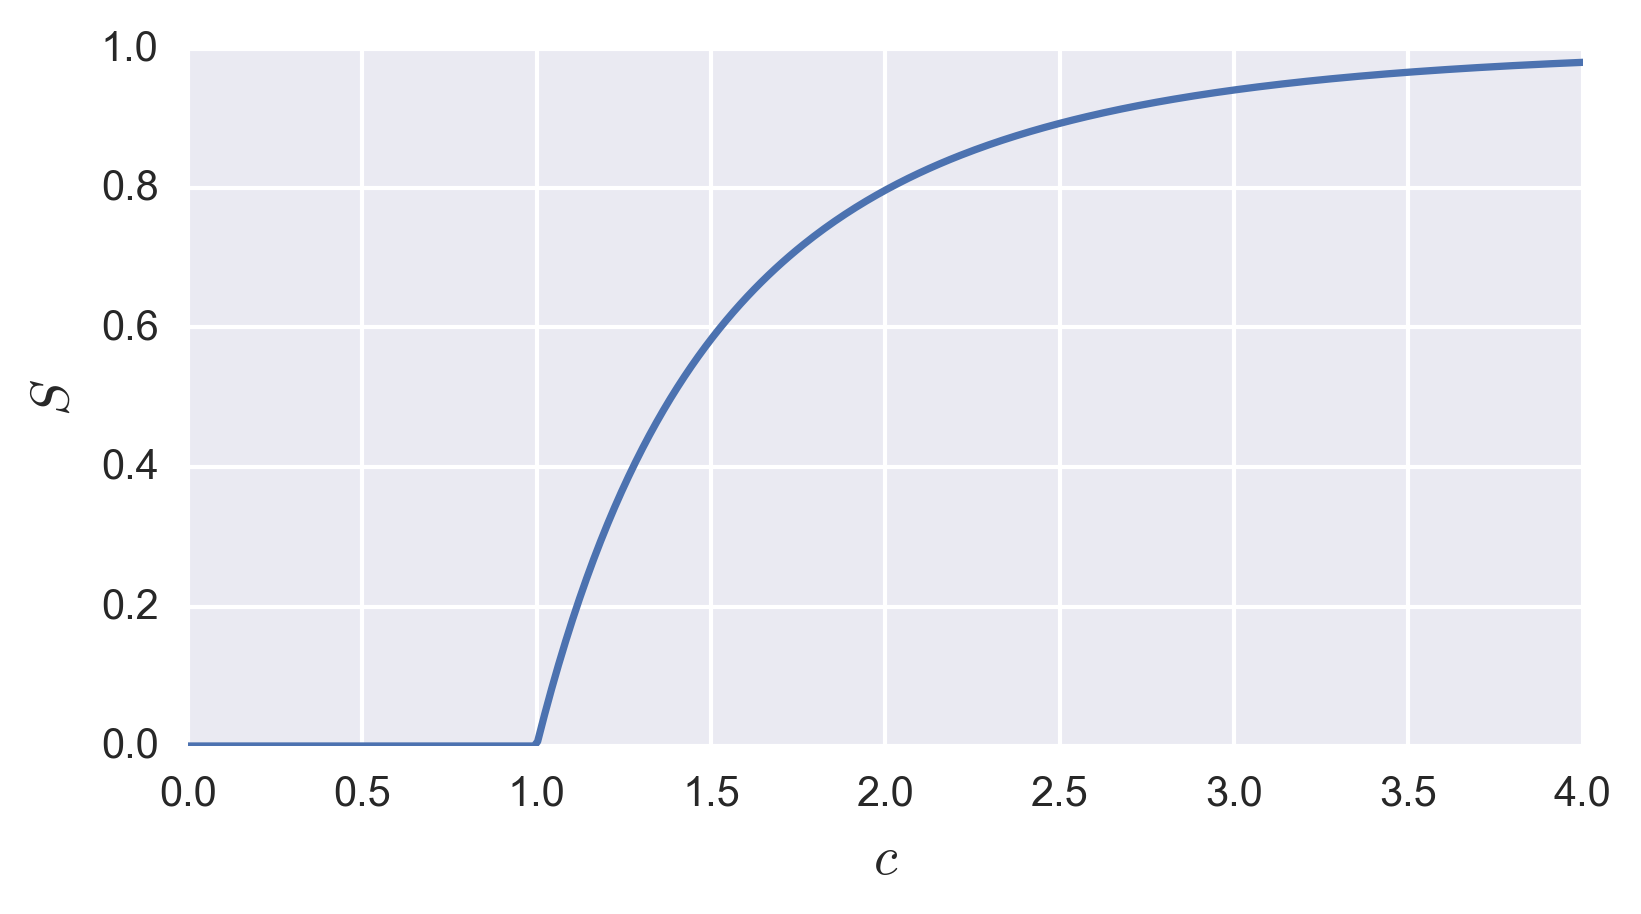
\includegraphics[]{figures/2_s_as_function_of_c.png}
	\caption{The fraction of the graph occupied by the giant component, $S$, as a function of the average expected degree $c$, and computed according to equation~\ref{eq:s_giant_component_lambert}. The phase transition at $c=1$ is well visible. For $c < 1$, no giant component is present, for $c>1$ it quickly occupies a dominating fraction of the network.}
	\label{fig:s_as_function_of_c}
\end{figure}

% subsection giant_component (end)








\subsection{Component sizes} % (fold)
\label{sub:component_sizes}


Generating functions.

The average size of $\mean{s}$ becomes 
\begin{equation}
	\mean{s} = \frac{1}{1-c-cS}
\end{equation}
with $S$ being the fractional size of the giant component, as given by equation~\ref{eq:s_giant_component_lambert}.

% subsection component_sizes (end)


% section random_graph_model (end)



\section{Generating functions} % (fold)
\label{sec:generating_functions}



We assume throughout this chapter that  follow~\cite{Newman:zFi032Kd}, which defines a set of generating functions for the probability distributions of some of the statistical properties of the graphs.
The basis of these is the function $G_0(x)$ for the probability distribution of vertex degrees $k$, defined as
\begin{equation}
G_0(x) = \sum_{k=0}^{\infty} p_k x^k
\end{equation}
where $p_k$ is the probability that a given vertex of the graph has degree $k$.

- normalization assumption ($G_0(1) = 1$)
- $G_0(x)$ is finite for all $|x| \le 1$

The derivatives of this function can be used to derive other statistical quantities.
For example, one can recover the probability $p_k$ by taking the $k^{th}$ derivative of the $G_0$
\begin{equation}
	p_k = \frac{1}{k!} \frac{d^k G_0}{dx^k} \Big|_{x=0}.
\end{equation}

Furthermore, one can obtain the average degree $z$ of the nodes in a graph 
\begin{equation}
	z = \mean{k} = \sum_k k p_k = G'_0(1)
\end{equation}

The function is given by the polylogarithm function
\begin{equation}
	\poly{n}{z} = \sum_{k=1}^{\infty} \frac{z^k}{k^n}
\end{equation}

\subsubsection{Component sizes} % (fold)
\label{ssub:component_sizes}

$H_1(x)$ follows the recursive condition
\begin{equation}
	H_1(x) = x G_1( H_1(x))
\end{equation}








\begin{equation}
\mean{s} = 1 + \frac{G'_0(1)}{1-G'_1(1)}	
\end{equation}




For a Poisson random graph







For a power law graph, this is given by
\begin{equation}
	G_1(x) = \frac{\poly{\tau-1}{xe^{-1/\kappa}}}{x\poly{\tau-1}{e^{-1/\kappa}}}
\end{equation}
and therefore
\begin{equation}
	G'_1(x) = \frac{\operatorname{Li}_{s - 2} \left(x e^{- 1/\kappa}\right)}
	               {x^{2} \operatorname{Li}_{s - 1}\left(e^{- 1/\kappa}\right)} -
	          \frac{\operatorname{Li}_{s - 1}\left(x e^{- 1/\kappa}\right)}
	               {x^{2} \operatorname{Li}_{s - 1}\left(e^{- 1/\kappa}\right)}
\end{equation}




In some networks, the degree distribution for large values is not quite a power law, while for small values it is. This is particularly appropriate when there are costs associated with having large degrees. For example, building and maintaining a large social network, or publishing papers with many people, requires time and energy, both of which are limited. Therefore, one cannot really expect to see the huge fluctuations that are predicted by power-law distributions. A related model is a power law with an exponential cut off, where the probability mass function is given by
\begin{equation}
	p_k = ck^{-\tau} e^{− k / A}, k \ge 1,
\end{equation}

for some large A. Thus, for k small compared to A the distribution looks like a power law, while for values that are large compared to A the exponential decay takes over.
We continue to discuss the notion of highly connected graph sequences.


% subsubsection component_sizes (end)Component sizes
% section generating_functions (end)



\section{Configuration model} % (fold)
\label{sec:configuration_model}

The configuration model is one of the most popular null models for the study of the statistical properties of networks.
It is inspired 

% section configuration_model (end){Configuration model}


% chapter graphs_and_networks (end)